\documentclass[../../../Bachelorarbeit.tex]{subfiles}
\begin{document}

\subsection{Funktionale Sicherheit} \label{sicherheit}
% \color{red}
% An sich nicht Teil des Bachelors. Muss also theoretisch nicht modelliert werden -> Absprache mit Herr Schäfer. Vielleicht trotzdem kurze Aufbereitung der Thematik, wenn Zeit !
Dieses Unterkapitel behandelt die funktionale Sicherheit des mehrachsigen Positioniersystems. Es wird eine Risikobeurteilung vorgenommen, die zu einer Handlungsempfehlung bei der fehlersicheren Inbetriebnahme des Systems führt. Der folgende Inhalt ist lediglich eine Zusammenfassung, die als Überblick dient. Die Mittel zur Minderung \bzw Vermeidung von Risiken gelten als vorgegeben. Ziel dieses Kapitels ist es nicht eine Risikoanalyse mit anschließender Modellierung von Sicherheitsmaßnahmen vorzunehmen.\\
\bigskip \newline
Grundsätzlich können zwei Gefahrenstellen am System erkannt werden. Dies ist zum Einen die Gefährdung von Personen durch einen elektrischen Schock und zum anderen die Gefahr der Verletzung durch die Bewegungen des Systems. Die Gefahrenbeurteilung kommt zu folgendem Ergebnis:\\
\bigskip \newline
\textbf{S Schwere der Verletzung}\\
S1 leichte (üblicherweise reversible Verletzung)\\
S2 ernste (üblicherweise irreversible Verletzung oder Tod)\\
\textbf{F Häufigkeit und/oder Dauer der Gefährdungsexposition}\\
F1 selten bis weniger häufig und/oder die Zeit der Gefährdungsexposition ist kurz\\
F2 häufig bis dauernd und/oder die Zeit der Gefährdungsexposition ist lang\\
\textbf{P Möglichkeit zur Vermeidung der Gefährdung oder Begrenzung des Schadens}\\
P1 möglich unter bestimmten Bedingungen\\
P2 kaum möglich

\begin{figure}[H]
    \centering
    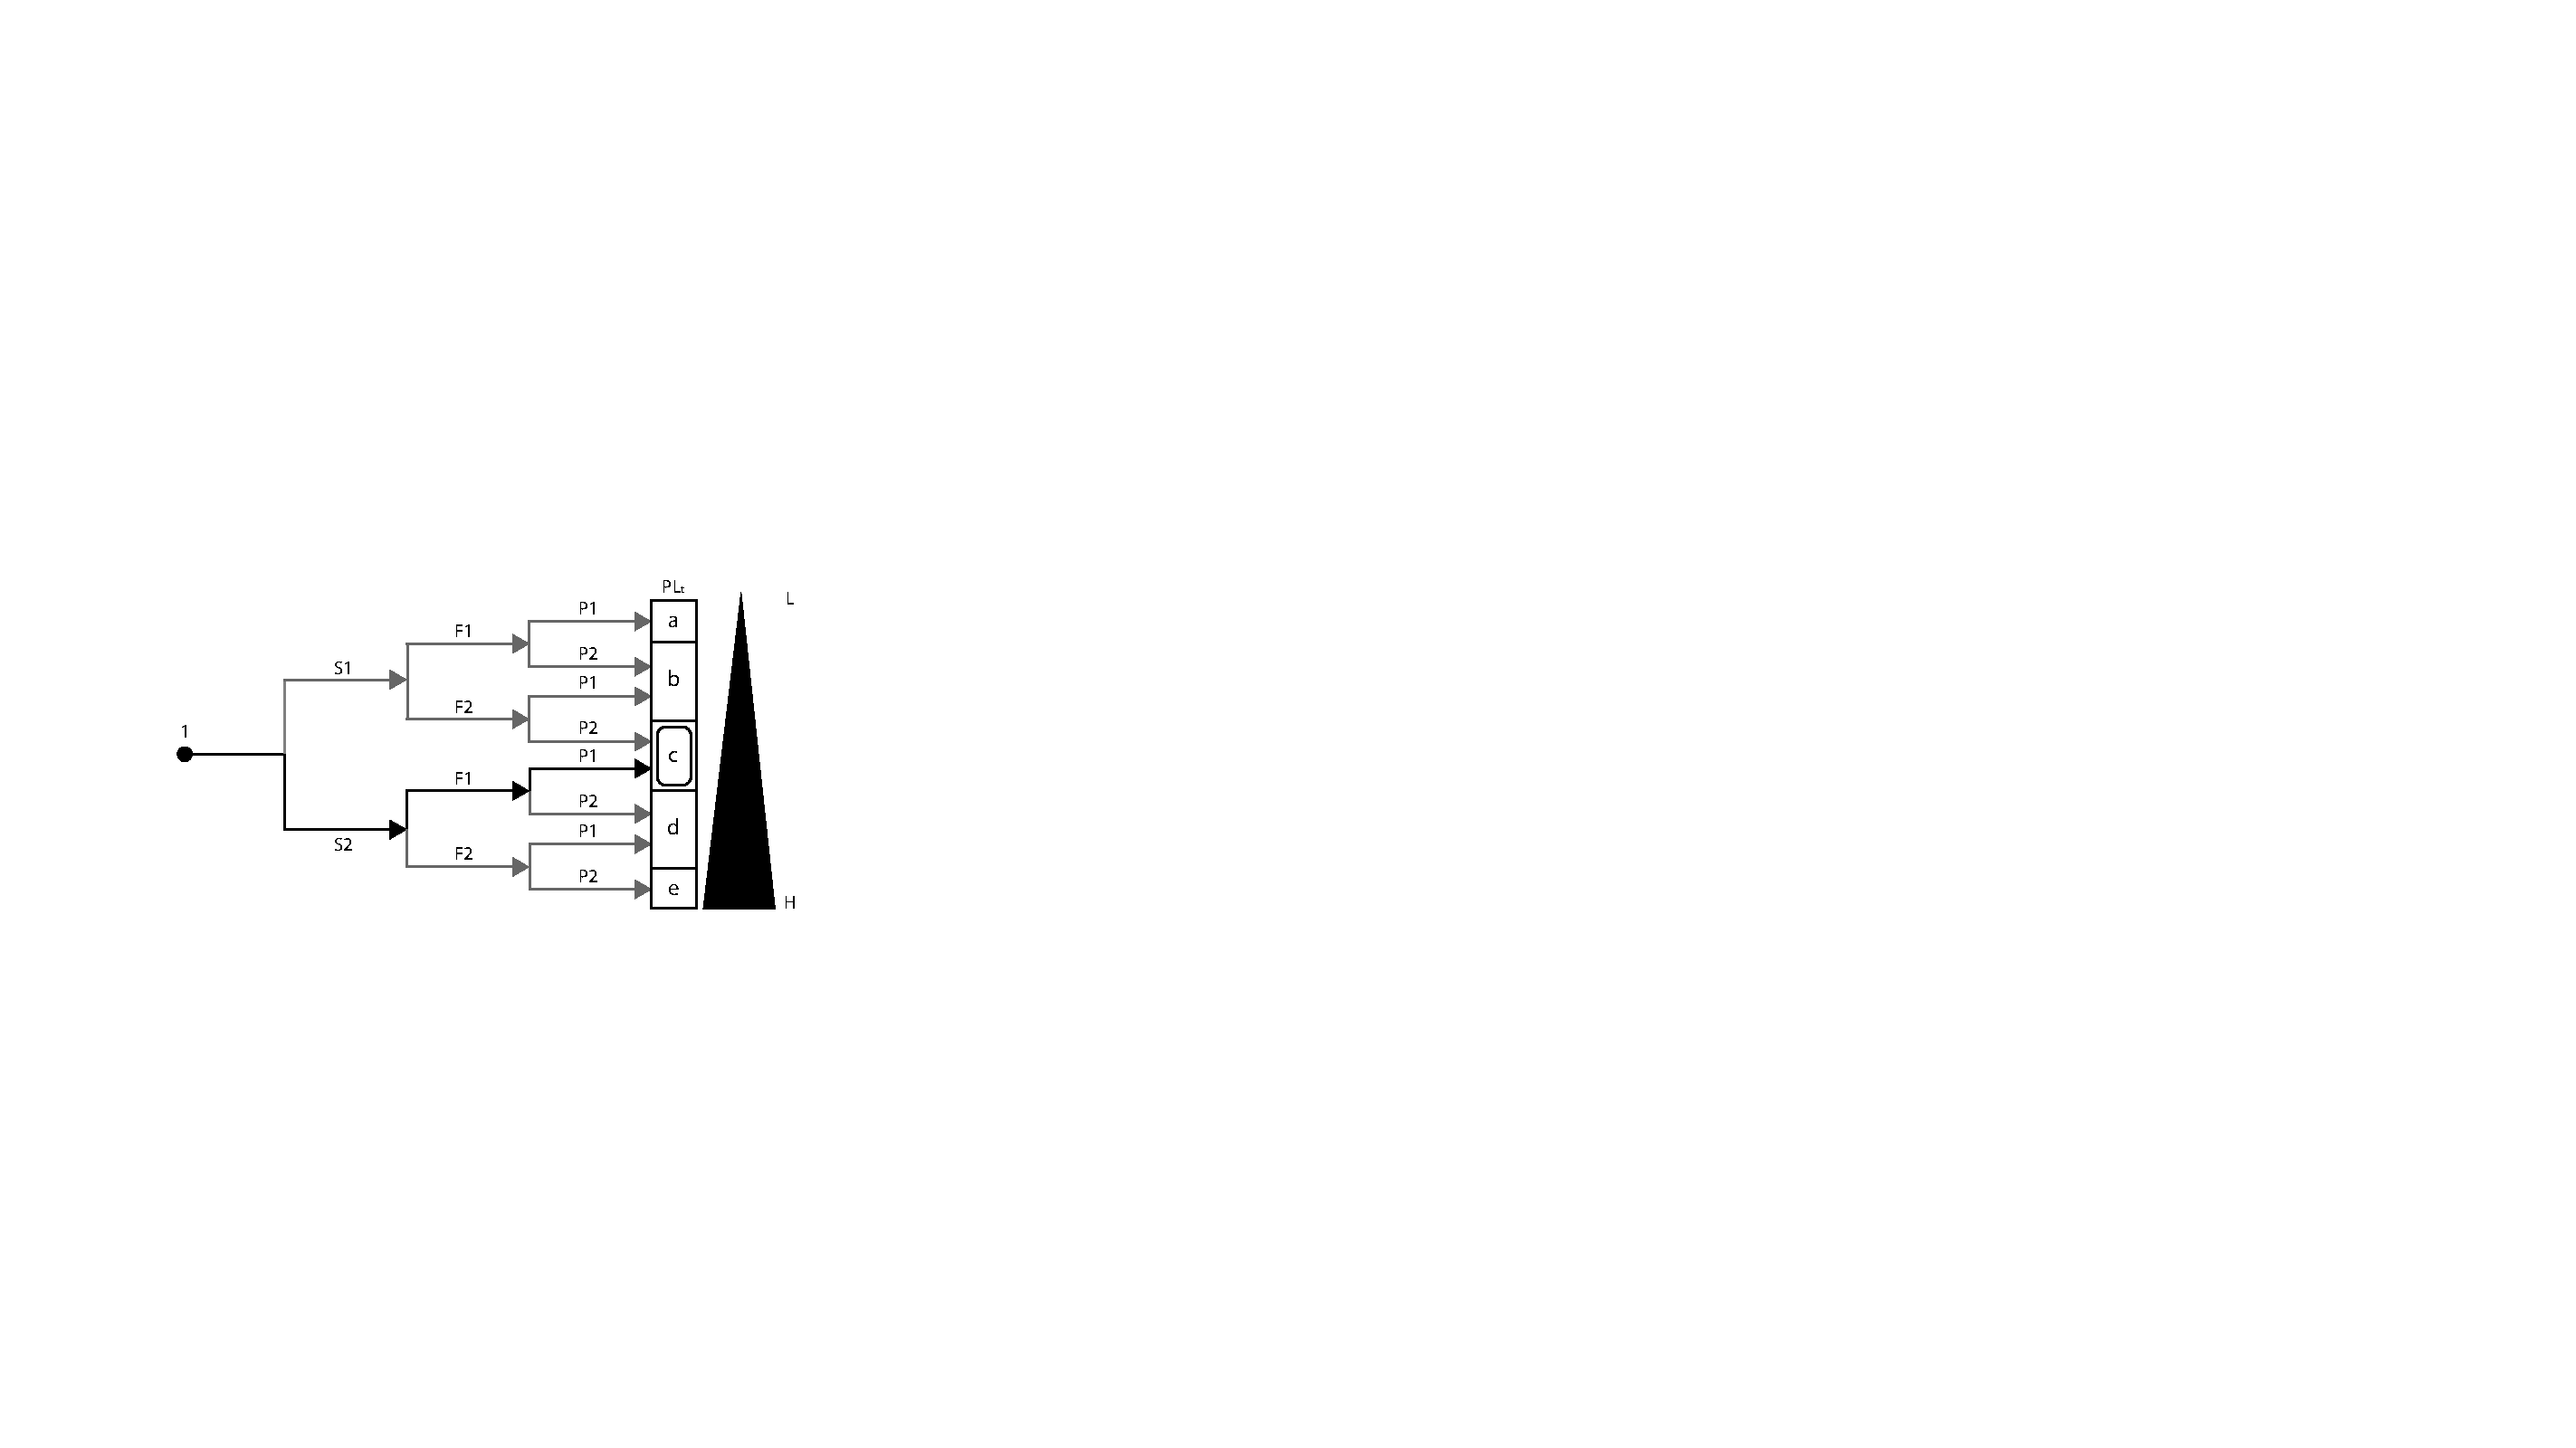
\includegraphics[width=0.7\textwidth]{Images/Risikograph.pdf}
    \caption[Risikograph]{Risikograph nach DIN EN ISO 13849-1 zum mehrachsigen Positioniersystem}
    \label{fig:my-img103}
\end{figure}

Zur Minderung der Risiken soll nun ein Lichtvorhang sowie mehrere Not-Halt Taster zur Anwendung kommen. Es gelten folgende vorgegebene Reaktionszeiten:\\
\bigskip \newline
Maximale Auslösezeit des Lichtvorhangs: 50 \si{ms}\\
Maximale Bremsdauer bei Not-Halt: 200 \si{ms}\\
Maximale Abschaltzeit des Servoreglers bei Not-Halt: 250 \si{ms}\\

Das System sei maximal sicher nach der Implementierung der aufgezählten Maßnahmen. Das bedeutet jedoch nicht, dass es zu 100\% sicher ist. Die Umsetzung der funktionalen Sicherheit ist in \autoref{implementation} dokumentiert.

% TODO: Hier muss noch mehr hin !!!

\end{document}